O programa foi testado de modo a ser possível estudar o comportamento da nossa resolução não só com puzzles de tamanho diferente, mas também com estratégias de pesquisa diferentes.
É de salientar que os resultados apresentados poderão diferir de máquina para máquina, devido aos diferentes tempos de processamento.

\subsection{Análise Dimensional}
O programa foi testado com problemas de 2 a 7 linhas.

\begin{figure}
    \centering
    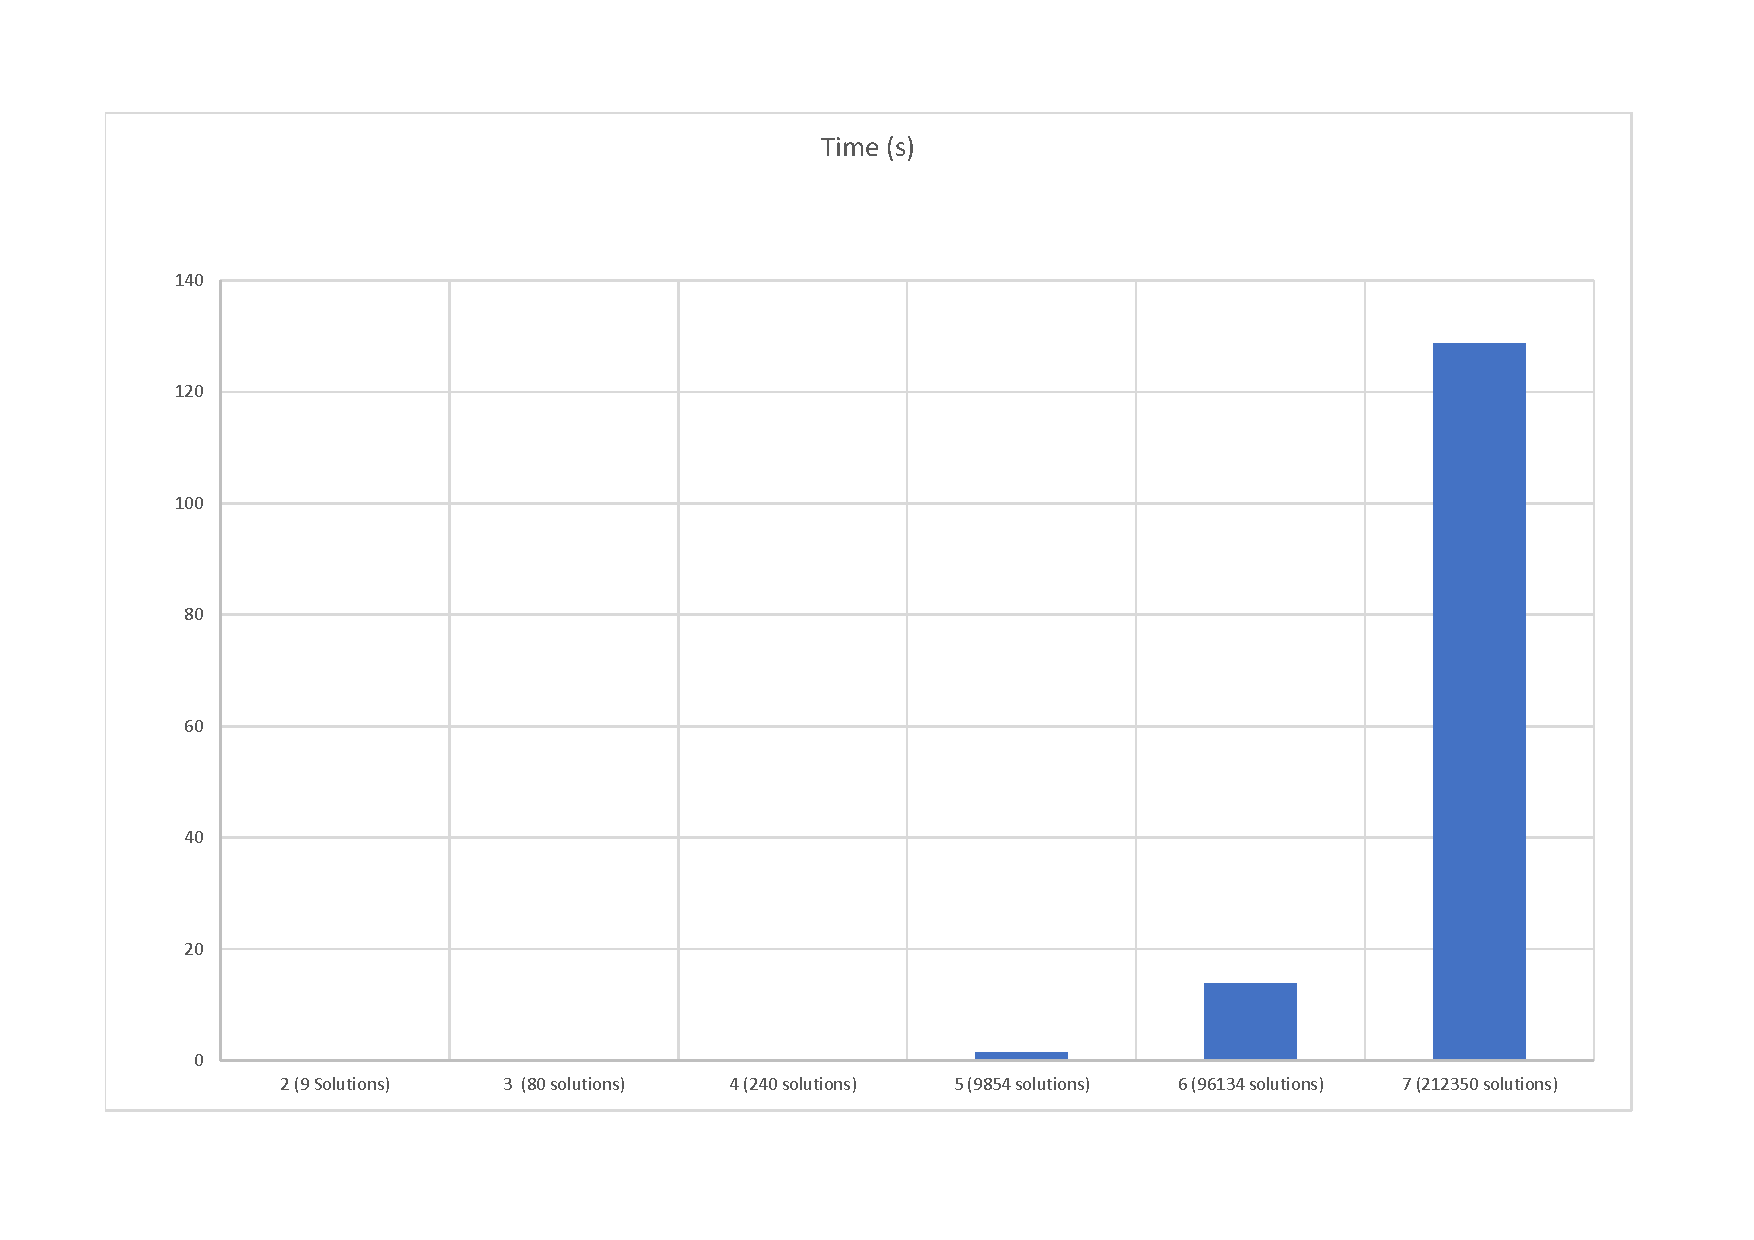
\includegraphics{size_graphs.pdf}
    \caption{Análise Dimensional}
    \label{fig: sizegraph}
\end{figure}

Como podemos observar pelo gráfico, o crescimento do tempo foi exponencial e por esta razão, não se testaram problemas de tamanho superior a 7 linhas.

\subsection{Estratégias de Pesquisa}
O programa foi testado com todas as combinações de heurísticas.

\begin{figure}
    \centering
    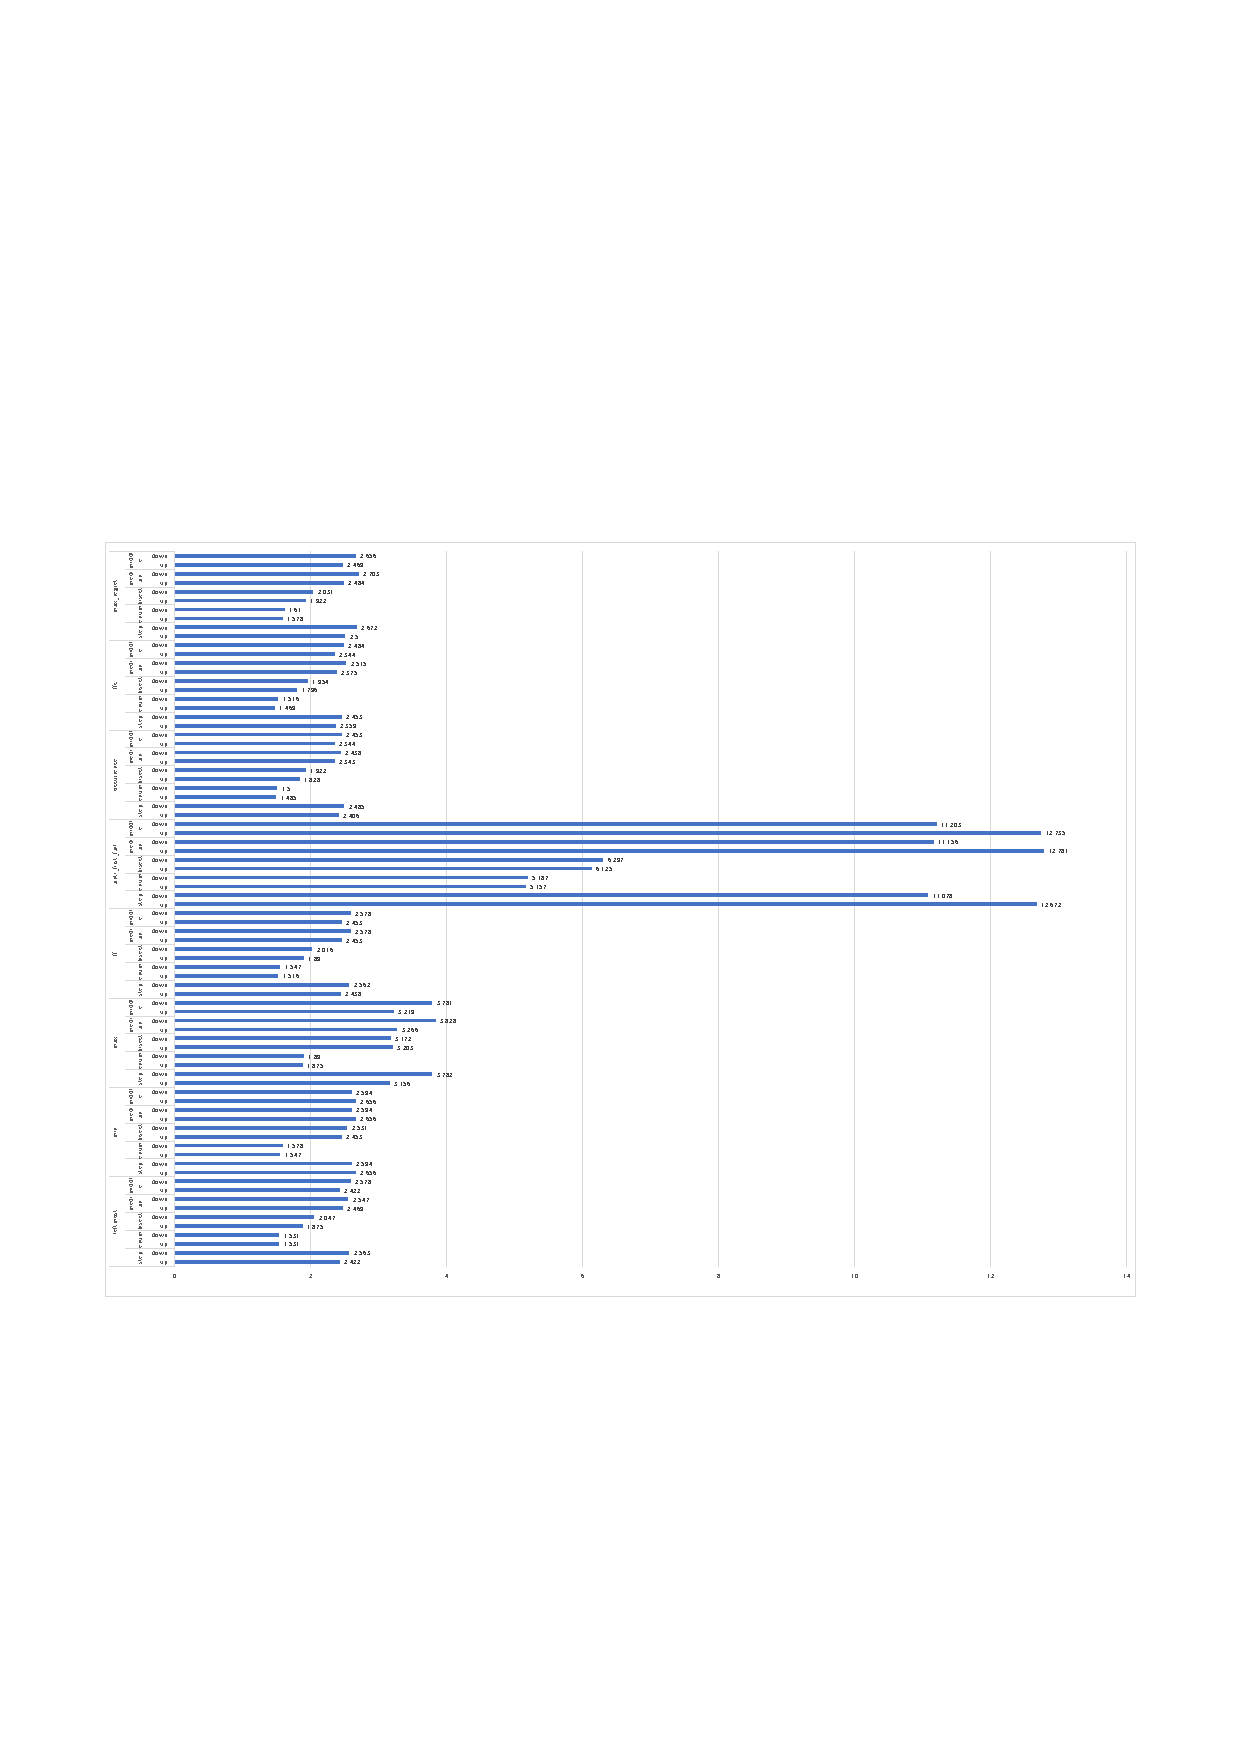
\includegraphics{heuristics.pdf}
    \caption{Análise temporal de estratégias de pesquisa}
    \label{fig: searchstrategy}
\end{figure}

Através da observação do gráfico, concluímos que a combinação mais eficiente seria \textbf{[ffc,enum,up]}.